
\clearpage
\section{User Management}

\begin{wrapfigure}[7]{l}{6.5cm}   % [x] Wie manche Zeile soll sich um die Grafik "brechen"
  \vspace{-35pt}      % Grundwert war 20; mit 30 schön oben beim Text ausgerichtet
  \begin{center}
    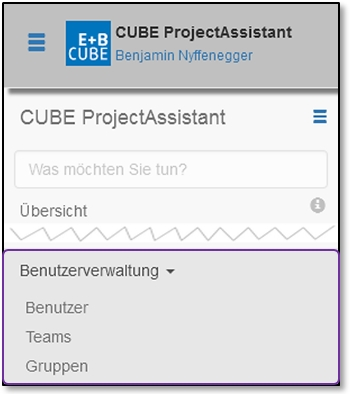
\includegraphics[width=1\linewidth]{../chapters/14_Benutzerverwaltung/pictures/14_Menu_Benutzerverwaltung.jpg}
  \end{center}
  \vspace{-20pt}
  \caption{Using the user management}
  \vspace{-10pt}
\end{wrapfigure}

In the menu on the left, select the 'User Management' menu item. The subitems 'User', 'Teams' and 'Groups' appear.

\vspace{\baselineskip}

User management is only accessible for users with the necessary access rights. It is used exclusively by administrators.

\vspace{5cm}  

\textbf{Overview:}

\vspace{\baselineskip}

\textbf{Users}: All users who have a point of contact with CUBE PA are registered here. Assignments to tags, meeting types, teams, etc. can be made here. In addition, it can be decided whether a user should get a CUBE PA access or only appear in selection fields (in meetings, procurements, document permissions, etc.). Users can be removed from the address list. An important 'control element' is the authorization roles which can be given to a user (e.g. administrator).

\vspace{\baselineskip}

\textbf{Teams}: Teams, to which users can be assigned, can be defined here (settings under User).

\vspace{\baselineskip}

\textbf{Groups}: Groups, to which users, teams, and also participants can be added, can be created here. In addition, a group can be assigned specific access rights (reading rights, writing rights, deleting rights).

% \clearpage
\subsection{Users}
\label{bkm:Ref445362390}

The user overview can be filtered or searched as seen with other overviews in CUBE PA. Listed users can be viewed or edited in the user management \col{(3)}. \textbf{It is however not possible to add users here. New entries (persons and companies) must be created in the address list (see chapter \ref{bkm:Ref443738751}).} \\

\vspace{\baselineskip}

The list shows when a user has last been logged into CUBE PA.

\begin{figure}[H]
\center{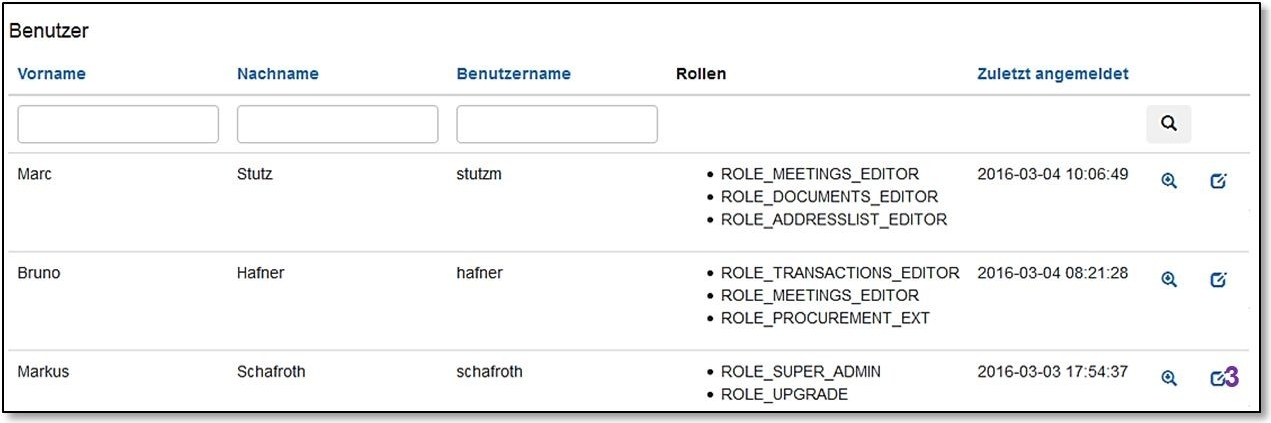
\includegraphics[width=1\linewidth]{../chapters/14_Benutzerverwaltung/pictures/14-1_Benutzeruebersicht.jpg}}
\caption{Overview of the user administration}
% \label{fig:speciation}
\end{figure}

The user management and the address list access the same data in the database. In the user management, the focus is directed to users who can log in to CUBE PA. As seen in the address list, adding a person to the address list is designed in such a way that the person \textbf{cannot} log in to CUBE PA. The check mark for 'enabled' is missing and needs to be added later in user management by an authorized person \col{(2)}:

\begin{figure}[H]
\center{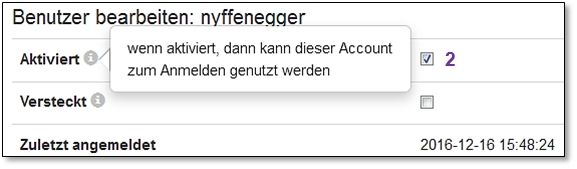
\includegraphics[width=.75\linewidth]{../chapters/14_Benutzerverwaltung/pictures/14-1_BenutzerAktivieren.jpg}}
\caption{Activating a user account}
% \label{fig:speciation}
\end{figure}

Click on the information icon 
\includegraphics[height=12pt]{/Icons/Info_Hinweis.jpg} to receive more information about the settings.

\vspace{-10pt}

% \clearpage
\subsubsection{Roles}
\label{bkm:Ref445361985}

The following roles can be assigned to a user:

\begin{tabular}{|p{7.5cm}|p{7.5cm}|} % {c | p{14cm} l} %{cl}
\hline
\textbf{Role} & \textbf{Type} \\
\hline	
ROLE\_IMPORT & ROLE\_USER \\
\hline
ROLE\_IMPORT\_PROJECT\_PLAN\_DATA & ROLE\_IMPORT \\
\hline
ROLE\_IMPORT\_TRANSACTION\_DATA & ROLE\_IMPORT \\
\hline
ROLE\_PROCUREMENT & ROLE\_USER \\
\hline
ROLE\_PROCUREMENT\_EXT & ROLE\_PROCUREMENT \\
\hline
ROLE\_TRANSACTIONS & ROLE\_USER \\
\hline
ROLE\_TRANSACTIONS\_EDITOR & ROLE\_TRANSACTIONS \\
\hline
ROLE\_MEETINGS & ROLE\_USER \\
\hline
ROLE\_MEETINGS\_EDITOR & ROLE\_MEETINGS \\
\hline
ROLE\_HUMANRESOURCES & ROLE\_USER \\
\hline
ROLE\_HUMANRESOURCES\_EDITOR & ROLE\_HUMANRESOURCES \\
\hline
ROLE\_DOCUMENTS & ROLE\_USER \\
\hline
ROLE\_DOCUMENTS\_EDITOR & ROLE\_DOCUMENTS \\
\hline
ROLE\_ADDRESSLIST\_EDITOR & ROLE\_USER \\
\hline
ROLE\_HANDBOOK\_EDITOR & ROLE\_USER \\
\hline
ROLE\_SUPER\_USER & ROLE\_HUMANRESOURCES\_EDITOR, ROLE\_MEETINGS\_EDITOR, \newline ROLE\_TRANSACTIONS\_EDITOR, \newline ROLE\_PROCUREMENT\_EXT, \newline ROLE\_DOCUMENTS\_EDITOR, \newline ROLE\_ADDRESSLIST\_EDITOR, \newline ROLE\_HANDBOOK\_EDITOR \\
\hline
ROLE\_ADMIN & ROLE\_USER, \newline ROLE\_ADDRESSLIST\_EDITOR \\
\hline
ROLE\_SUPER\_ADMIN & ROLE\_ADMIN, \newline ROLE\_IMPORT\_PROJECT\_PLAN\_DATA, ROLE\_IMPORT\_TRANSACTION\_DATA, ROLE\_PROCUREMENT\_EXT,
\newline ROLE\_MEETINGS, \newline ROLE\_MEETINGS\_EDITOR, \newline ROLE\_TRANSACTIONS\_EDITOR, \newline ROLE\_HUMANRESOURCES\_EDITOR,
\newline ROLE\_DOCUMENTS\_EDITOR, \newline ROLE\_ADDRESSLIST\_EDITOR, \newline ROLE\_HANDBOOK\_EDITOR \\
\hline
ROLE\_UPGRADE & ROLE\_USER \\
\hline
\end{tabular}

\begin{itemize}
\item
The role type~'ROLE\_USER' gives the lowest level of access rights and is assigned automatically to a user in their first log in.
\item
ROLE\_A: ROLE\_B: This role assignment means that the user with role A also has the role B.
\item
ROLE\_X: [ROLE\_Y, ROLE\_Z]: This role assignment means that the user with role X also has the roles between brackets (Y and Z).
\end{itemize}

'Edit user' overview:

\vspace{\baselineskip}
\vspace{\baselineskip}

\begin{wrapfigure}[7]{r}{9cm}
\vspace{-55pt}
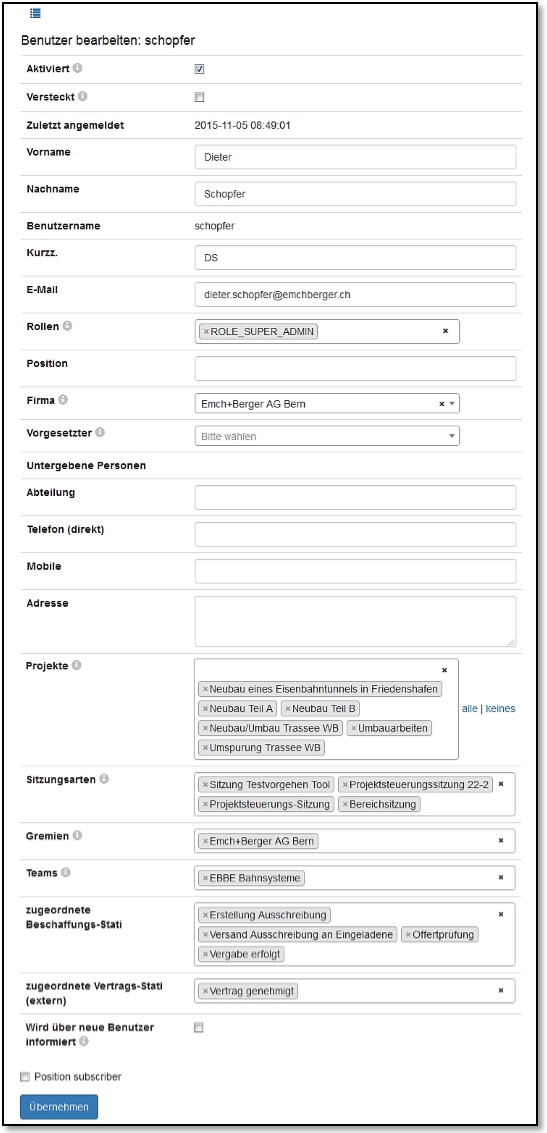
\includegraphics[height=185mm]{../chapters/14_Benutzerverwaltung/pictures/14-1-1_BenutzerBearbeiten.jpg}
% \caption{Status ändern}
\end{wrapfigure}

\begin{small}
\begin{raggedright}

The created user can log in to CUBE PA.

\vspace{\baselineskip}

\mbox{The user should not appear,} 
\mbox{in the address list}
and in the selection fields

\vspace{\baselineskip}

Assigning the different CUBE PA \
roles (see chapter \ref{bkm:Ref445361985})

\vspace{\baselineskip}
\vspace{\baselineskip}
\vspace{\baselineskip}

The users can be assigned

\vspace{\baselineskip}

\begin{itemize}
\item tags
\vspace{\baselineskip}
\vspace{\baselineskip}
\item meeting types
\vspace{\baselineskip}
\item committees
\item teams
\item procurement steps
\item and statuses in \newline the procurement function
\end{itemize}

\vspace{\baselineskip}



\end{raggedright}
\end{small}

\raggedright{}

\clearpage
\textbf{Information regarding functions}

\begin{figure}[H]
\center{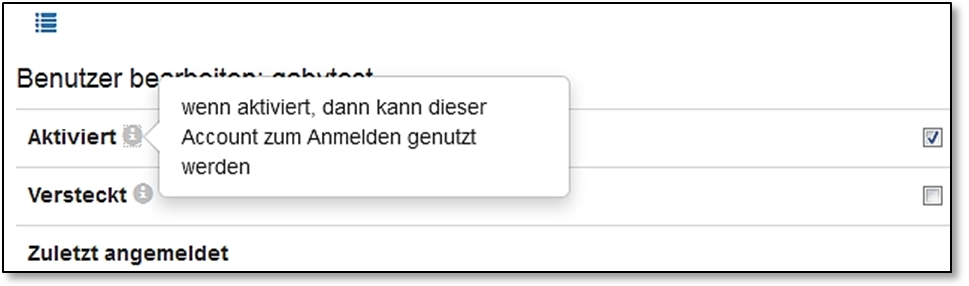
\includegraphics[width=0.6\linewidth]{../chapters/14_Benutzerverwaltung/pictures/14-1-1_Funktionshinweise.jpg}}
\caption{Function hints}
% \label{fig:speciation}
\end{figure}

An 'i' symbol 
\includegraphics[height=12pt]{/Icons/Info_Hinweis.jpg} can be found next to different fields. Click on the symbol to get information about the functions of the corresponding fields.

\subsection{Teams}

Teams that are created here can be assigned users (see chapter \ref{bkm:Ref445362390}).

\begin{figure}[H]
\center{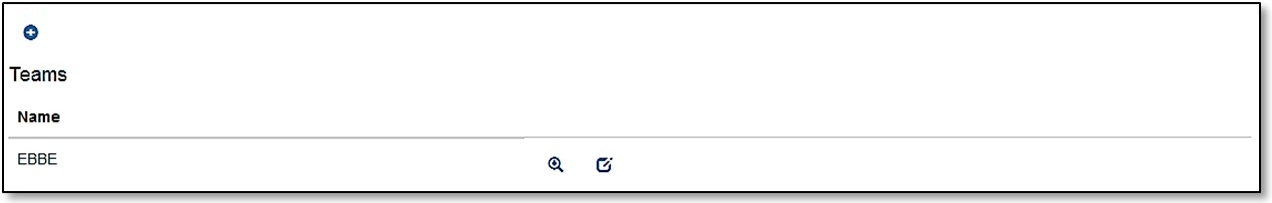
\includegraphics[width=1\linewidth]{../chapters/14_Benutzerverwaltung/pictures/14-2_TeamsUebersicht.jpg}}
\caption{Overview of the created teams}
% \label{fig:speciation}
\end{figure}

\begin{figure}[H]
\center{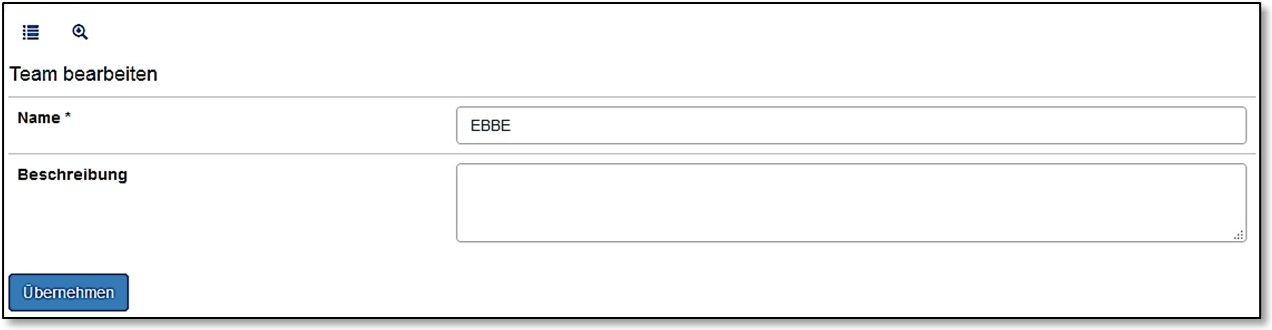
\includegraphics[width=1\linewidth]{../chapters/14_Benutzerverwaltung/pictures/14-2_TeamsBearbeiten.jpg}}
\caption{Team editing mode}
% \label{fig:speciation}
\end{figure}

\clearpage
\subsection{Groups}

Groups, to which users, teams, and also participants can be added, can be created here. In addition, a group can be assigned specific access rights (reading rights, writing rights, deleting rights).

\begin{figure}[H]
\center{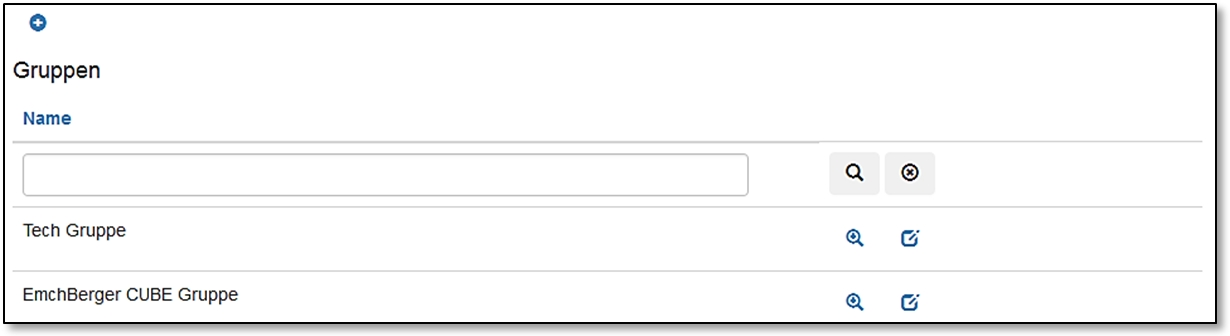
\includegraphics[width=1\linewidth]{../chapters/14_Benutzerverwaltung/pictures/14-3_GruppenUebersicht.jpg}}
\caption{Group overview}
% \label{fig:speciation}
\end{figure}

\begin{figure}[H]
\center{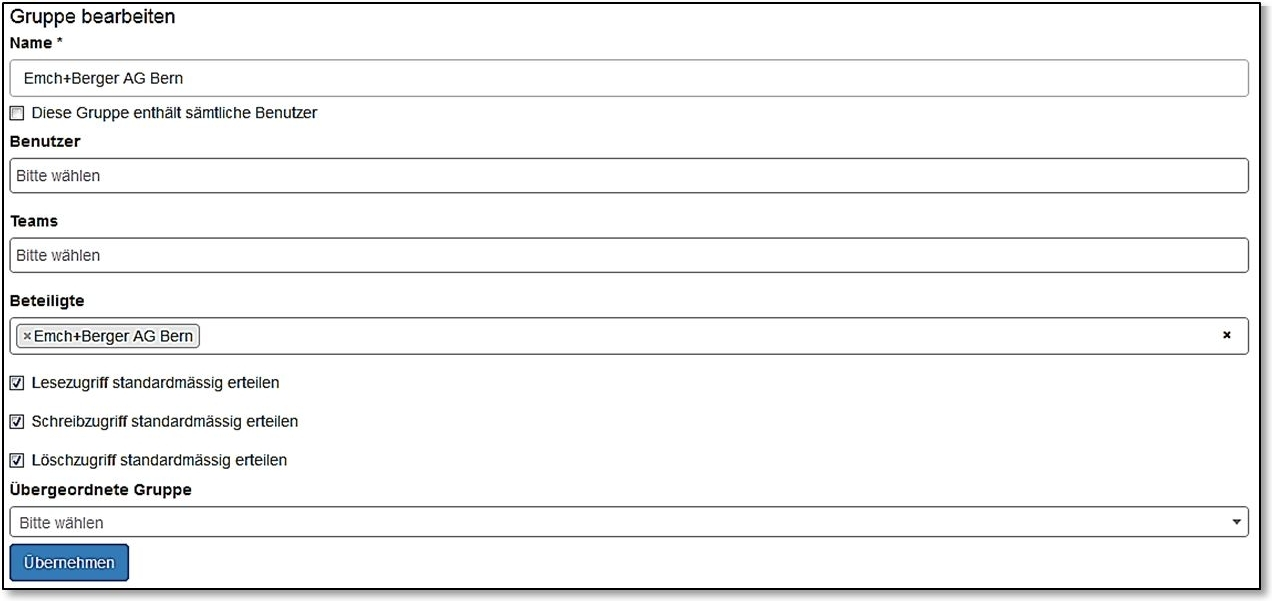
\includegraphics[width=1\linewidth]{../chapters/14_Benutzerverwaltung/pictures/14-3_GruppenBearbeiten.jpg}}
\caption{Group editing mode}
% \label{fig:speciation}
\end{figure}
